\clearpage
\section{Service Equipment, Incense, and Vesture Preparation}
\PCDPlateHeader{Plate VI --- Processional and Service Equipment}{Not to common scale}
\ifdefined\TriptychPrintEdition
\begin{center}
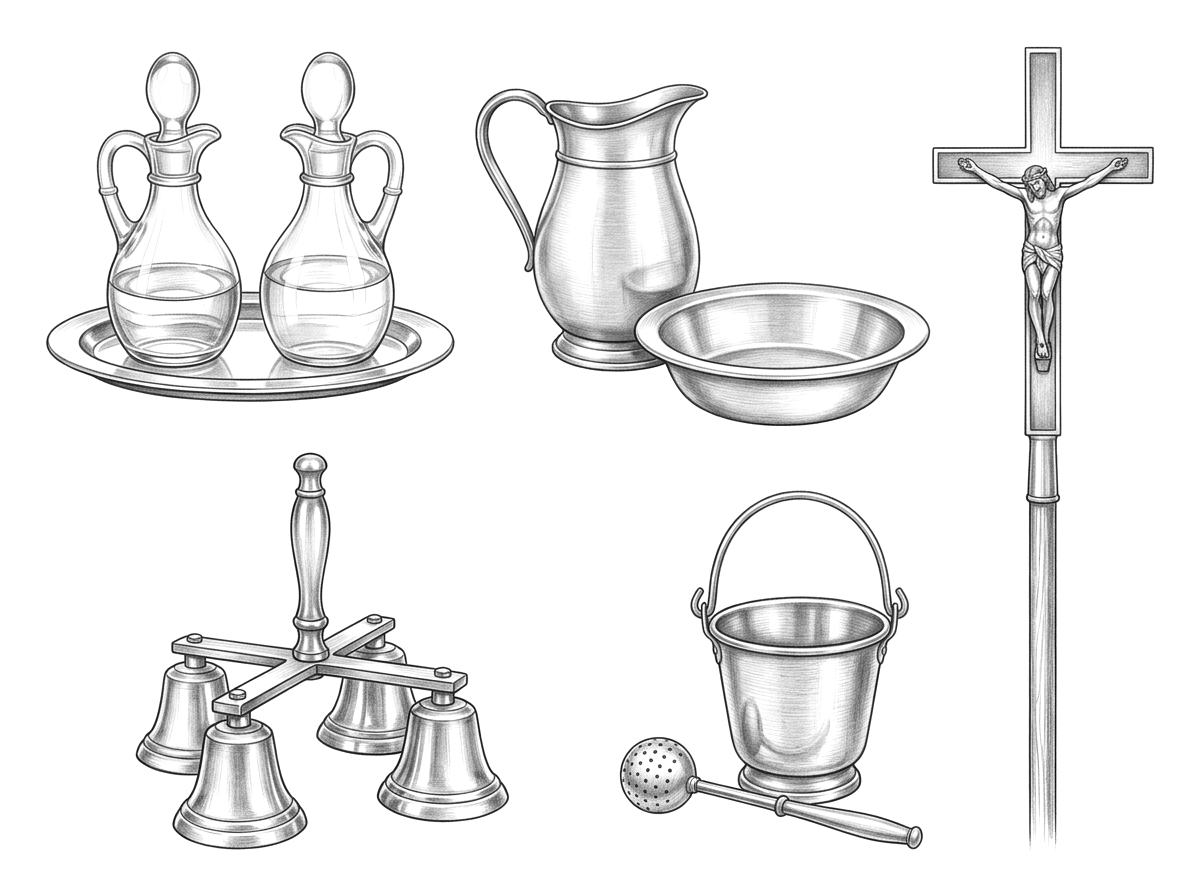
\includegraphics[width=0.92\linewidth,height=3.55in,keepaspectratio]{liturgy/roman-rite/postconciliar/2008-latin-2011-us-english/reference/roman-sanctuary-dictionary/shared/artwork/graphite/pc-art-06-service-cruets-bells.png}
\end{center}
\PCDPositionKey{Top left: paired glass wine and water Cruets with stoppers on a tray; top center: Lavabo pitcher and shallow finger basin; top right: Processional Cross bearing the sculpted corpus of Christ on a staff; bottom left: four-cup mounted brass Sanctuary Bell; bottom right: holy-water Aspersorium bucket and perforated metal Aspergillum.}
\else
\textbf{Visual Plate Summary (Plate VI --- Processional and Service Equipment, Not to common scale):} Five-object monochrome graphite service equipment study: top left, two stoppered transparent glass cruets for wine and water resting on an oval metal tray; top center, a metal lavabo pitcher beside a shallow round finger basin; top right, a tall processional cross on a wooden staff bearing the sculpted figure of Christ crucified; bottom left, a traditional four-bell mounted brass sanctuary hand bell; bottom right, a metal holy-water aspersorium bucket with bail handle and perforated spherical-head aspergillum resting beside it.

\textbf{Reading order and object placement:} Top left: paired glass wine and water Cruets with stoppers on a tray; top center: Lavabo pitcher and shallow finger basin; top right: Processional Cross bearing the sculpted corpus of Christ on a staff; bottom left: four-cup mounted brass Sanctuary Bell; bottom right: holy-water Aspersorium bucket and perforated metal Aspergillum.
\fi

\label{pc-obj-processional-cross}
\PCDEntryHead{Processional Cross}{Crux processionalis}{required}{N25}
\PCDField{Also called}{Altar Cross; Crucifix; \textit{Crux cum figura Christi crucifixi}}
Ensure that a cross bearing a clear figure of Christ crucified is prepared for the entrance procession or already stationed visibly on or near the altar (GIRM 117, 308). Check that the socket joint is tight and that the sanctuary floor stand is weighted, unobstructed, and does not duplicate an existing altar crucifix (GIRM 122).

\PCDField{Plate position and norm}{Top right, bearing sculpted corpus on wooden staff (Plate VI); altar cross at center (Plate I) (Universal Roman law)}
\PCDField{Placement and use}{During the entrance procession, an instituted acolyte or altar server carries the processional cross between two ministers bearing lighted candles (GIRM 120b). On reaching the sanctuary, the cross may be set in a floor stand near the altar to serve as the altar cross, in which case it must be the only cross present; otherwise it is placed away in a dignified spot while a separate crucifix remains clearly visible on or near the altar (GIRM 117, 122, 308). It is fitting that the cross with the figure of Christ crucified remain near the altar even outside liturgical celebrations (GIRM 308).}
\PCDField{Prepared and handled by}{Prepares: Sacristan, Altar server. Ministers in use: Instituted acolyte, Altar server.}
\PCDSafety{Do not bow or genuflect while holding the processional cross (GIRM 274), both to honor the rubric and to prevent the tall staff from pitching forward. Keep the staff clear of low doorways and hanging lights, and confirm that its weighted floor stand is level and stable before releasing it.}
\PCDEntryRule

\label{pc-obj-altar-candles}
\PCDEntryHead{Altar Candles}{Candelabra cum cereis}{required}{N26}
\PCDField{Also called}{Altar Candlesticks; Processional Candles; \textit{Cerei}; \textit{Candelabra}}
Set out the required number of trimmed wax or oil candles (two, four, or six, and seven when the Diocesan Bishop presides, GIRM 117) on or around the altar without blocking sightlines across the mensa (GIRM 307). Inspect oil followers or wax tubes for adequate fuel, clean hardened wax from drip shields, and keep a taper lighter and snuffer ready in the sacristy.

\PCDField{Plate position and norm}{See Plate I, flanking the freestanding altar (Universal Roman law)}
\PCDField{Placement and use}{At every celebration of Mass, lighted candles are placed on or around the altar: at least two candlesticks, or four or six especially for Sunday Mass and Holy Days of Obligation, and seven when the Diocesan Bishop celebrates (GIRM 117). Candlesticks are arranged harmoniously with the architecture of the altar and sanctuary so that they never obstruct the assembly's clear view of what takes place upon the mensa (GIRM 307). Two lighted candles also accompany the processional cross at the entrance procession and flank the Book of the Gospels during the Gospel procession and proclamation at the ambo (GIRM 120b, 133, 175).}
\PCDField{United States norm}{GIRM 117 and 307 are universal Roman norms without a separate territorial insertion for the United States. Guidance of the USCCB Committee on Divine Worship maintains real living flames of wax or oil rather than electric lights.}
\PCDField{Prepared and handled by}{Prepares: Sacristan, Altar server. Ministers in use: Instituted acolyte, Altar server.}
\PCDSafety{Keep open flames well clear of hair, albs, ribbons, vestments, and the pages of the Roman Missal. Carry processional candles strictly upright, watch for dripping hot wax, and extinguish every flame with a brass snuffer rather than blowing melted wax onto the white altar cloth.}
\PCDField{Distinguish from}{Sanctuary Lamp}
\PCDEntryRule

\label{pc-obj-sanctuary-bells}
\PCDEntryHead{Sanctuary Bells}{Campanula}{optional}{N27}
\PCDField{Also called}{Altar Bell; Sanctus Bell; \textit{Parva campanula}}
Set the clean, intact sanctuary bell on the credence table or at the servers' station whenever parish custom uses it (GIRM 150). Check that the clappers hang freely and are securely pinned, and remove all sanctuary bells from the sanctuary after the Gloria on Holy Thursday evening until the Easter Vigil.

\PCDField{Plate position and norm}{Bottom left, four-cup mounted brass altar bell (Plate VI) (Documented custom)}
\PCDField{Placement and use}{When used according to local custom, the sanctuary bell rests on the credence table or beside the servers' kneeling place before the Eucharistic Prayer. Shortly before the consecration---customarily as the priest extends his hands over the gifts at the epiclesis---an instituted acolyte or altar server may give a crisp signal on the bell, and likewise ring it at each showing of the consecrated Host and Chalice (GIRM 150). Bells remain silent from the conclusion of the Gloria at the Evening Mass of the Lord's Supper on Holy Thursday until the Gloria of the Easter Vigil.}
\PCDField{Prepared and handled by}{Prepares: Sacristan, Altar server. Ministers in use: Altar server, Instituted acolyte.}
\PCDEntryRule

\label{pc-obj-aspergillum-aspersorium}
\PCDEntryHead{Aspergillum and Aspersorium}{Aspergillum et aspersorium}{optional}{N28}
\PCDField{Also called}{Holy-Water Sprinkler and Bucket; Holy-Water Vessel; \textit{Vas aquae benedicendae}; \textit{Vas aquae benedictae}}
Clean and dry the interior liner of the aspersorium regularly so mineral deposits do not accumulate, and inspect the perforated head of the aspergillum to ensure its internal sponge (if fitted) is clean and free of mildew. Set fresh clean water in the vessel on the credence table before any Mass using the Sunday sprinkling rite (GIRM 51, 118c), and pour any remaining blessed water after use into the sacrarium or clean earth.

\PCDField{Plate position and norm}{Bottom right, holy-water bucket and perforated sprinkler (Plate VI) (Universal Roman law)}
\PCDField{Placement and use}{On Sundays, especially during Easter Time, the Order for the Blessing and Sprinkling of Water may replace the ordinary Penitential Act within the Introductory Rites of Mass (GIRM 51; Roman Missal, Appendix II). When the sprinkling rite is scheduled, the clean vessel of water to be blessed (or already blessed, as at the Easter Vigil) is prepared with the sprinkler on the credence table (GIRM 118c). The priest---vested in his chasuble---blesses the water, sprinkles himself and the ministers, and walks through the church sprinkling the faithful while a deacon or server carries the bucket beside him. The same paired instruments serve at funerals, church blessings, and sacramentals in the Book of Blessings.}
\PCDField{Prepared and handled by}{Prepares: Sacristan, Altar server. Ministers in use: Bishop, Priest, Deacon.}
\PCDSafety{Fill the bucket only half to two-thirds full so water does not slosh over the rim onto stone or polished sanctuary steps and create a slipping hazard for ministers and communicants.}
\PCDField{Distinguish from}{Cruets, Baptismal Font}
\PCDEntryRule

\clearpage
\PCDPlateHeader{Plate VII --- Incense Equipment}{Not to common scale}
\ifdefined\TriptychPrintEdition
\begin{center}
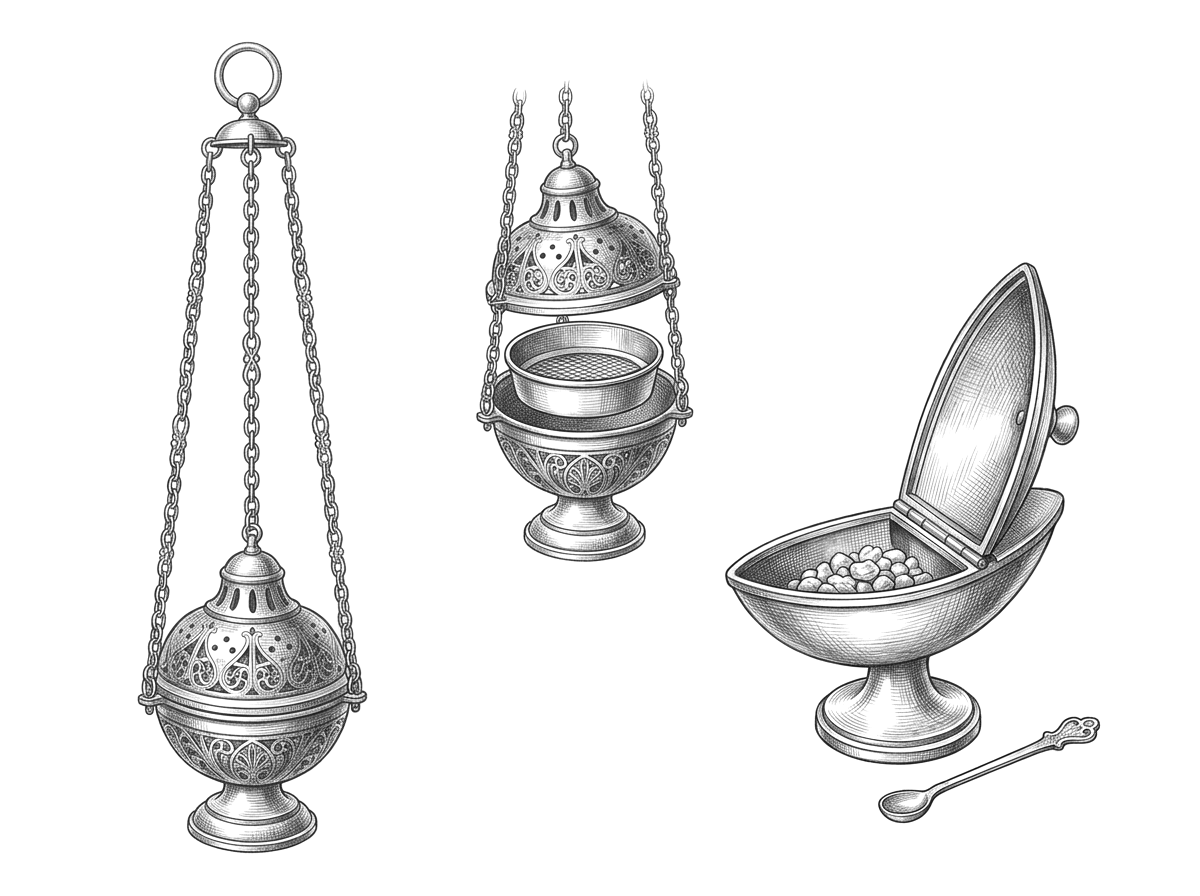
\includegraphics[width=0.92\linewidth,height=3.55in,keepaspectratio]{liturgy/roman-rite/postconciliar/2008-latin-2011-us-english/reference/roman-sanctuary-dictionary/shared/artwork/graphite/pc-art-07-incense-set.png}
\end{center}
\PCDPositionKey{Left: closed metal Thurible suspended on outer rim chains (two visible in profile) and one central lid-lifting chain; center: detail of raised perforated dome revealing removable inner charcoal fire-pan; right: footed Incense Boat (navicula) with hinged half-lid open showing resin grains, accompanied by its metal spoon.}
\else
\textbf{Visual Plate Summary (Plate VII --- Incense Equipment, Not to common scale):} Three-part monochrome graphite incense study: left, a classical footed metal thurible hanging vertically from its top ring on outer rim chains (two visible in profile) and a central lid-lifting chain with perforated domed cover closed; center, a sectional open view with the dome lifted to expose the removable circular charcoal fire-pan; right, a pedestal-footed boat-shaped incense boat with hinged half-lid open showing resin incense grains, paired with a small long-handled metal spoon.

\textbf{Reading order and object placement:} Left: closed metal Thurible suspended on outer rim chains (two visible in profile) and one central lid-lifting chain; center: detail of raised perforated dome revealing removable inner charcoal fire-pan; right: footed Incense Boat (navicula) with hinged half-lid open showing resin grains, accompanied by its metal spoon.
\fi

\label{pc-obj-thurible}
\PCDEntryHead{Thurible}{Turibulum}{optional}{N29}
\PCDField{Also called}{Censer; \textit{Thuribulum}}
Keep the removable fire-pan free of built-up resin slag and inspect chain links, ring clasps, and dome vents before every solemnity so no chain snaps mid-swing. Provide quick-lighting or briquette charcoal, metal tongs, a safe heatproof lighter, a stable stand, and a lidded fireproof metal ash bucket in the sacristy for safe cooling after Mass.

\PCDField{Plate position and norm}{Left (closed on chains) and center inset (dome lifted revealing inner charcoal fire-pan) (Plate VII) (Universal Roman law)}
\PCDField{Placement and use}{Incense may be used optionally in any form of Mass at five appointed moments: during the entrance procession, at the start of Mass to incense the cross and altar, at the Gospel procession and proclamation, after the bread and chalice are placed on the altar to incense the offerings, cross, altar, priest, and people, and at the showing of the Host and Chalice after the consecration (GIRM 120a, 133, 144, 150, 276). The priest imposes incense onto the charcoal and blesses it silently with the Sign of the Cross (GIRM 277). Incensation follows the rhythmic swing pattern of GIRM 277---three swings (tribus ductibus) for the Blessed Sacrament, a relic of the True Cross, images of the Lord, the offerings, the altar cross, the Book of the Gospels, the paschal candle, the priest, and the people; two swings (duobus ductibus) for relics and images of the Saints; and continuous single swings while walking around the altar (each ductus being executed as a paired double swing in Roman ceremonial custom, Caeremoniale Episcoporum 92)---framed by a profound bow before and after except when incensing the altar and offerings.}
\PCDField{Prepared and handled by}{Prepares: Sacristan, Altar server, Instituted acolyte. Ministers in use: Bishop, Priest, Deacon, Instituted acolyte, Altar server.}
\PCDSafety{Handle burning charcoal exclusively with metal tongs, never with bare fingers. Keep the hot bowl and chains clear of vestments, white altar linens, and narrow aisles, swing only with controlled short wrist movements, and empty spent coals into a dedicated fireproof metal ash vessel rather than an ordinary trash bin.}
\PCDField{Distinguish from}{Sanctuary Lamp}
\PCDEntryRule

\label{pc-obj-incense-boat}
\PCDEntryHead{Incense Boat}{Navicula}{optional}{N30}
\PCDField{Also called}{Incense Boat and Spoon; \textit{Navicula cum cochleari}}
Fill the incense boat about halfway with dry, properly sized resin grains before Mass---overfilling makes the lid jam and causes spills during processions. Store the companion spoon securely with the boat and brush away fine resin dust from the hinge periodically so the cover opens smoothly.

\PCDField{Plate position and norm}{Right, boat-shaped vessel with hinged half-lid open and spoon beside base (Plate VII) (Universal Roman law)}
\PCDField{Placement and use}{Whenever incense is employed during Mass, Benediction, or solemn Liturgy of the Hours (GIRM 120, 276--277), the incense boat accompanies the thurible. A dedicated boat-bearer---or the thurifer holding the boat in the left hand when serving alone---presents the opened vessel to the priest or deacon so that the priest may spoon resin grains onto the hot coals and bless them silently with the Sign of the Cross (GIRM 277).}
\PCDField{Prepared and handled by}{Prepares: Sacristan, Altar server. Ministers in use: Priest, Deacon, Instituted acolyte, Altar server.}
\PCDEntryRule

\clearpage
\PCDPlateHeader{Plate VIII --- Ordained Vesture at Mass}{Standing figures to common scale; insets not to scale}
\ifdefined\TriptychPrintEdition
\begin{center}
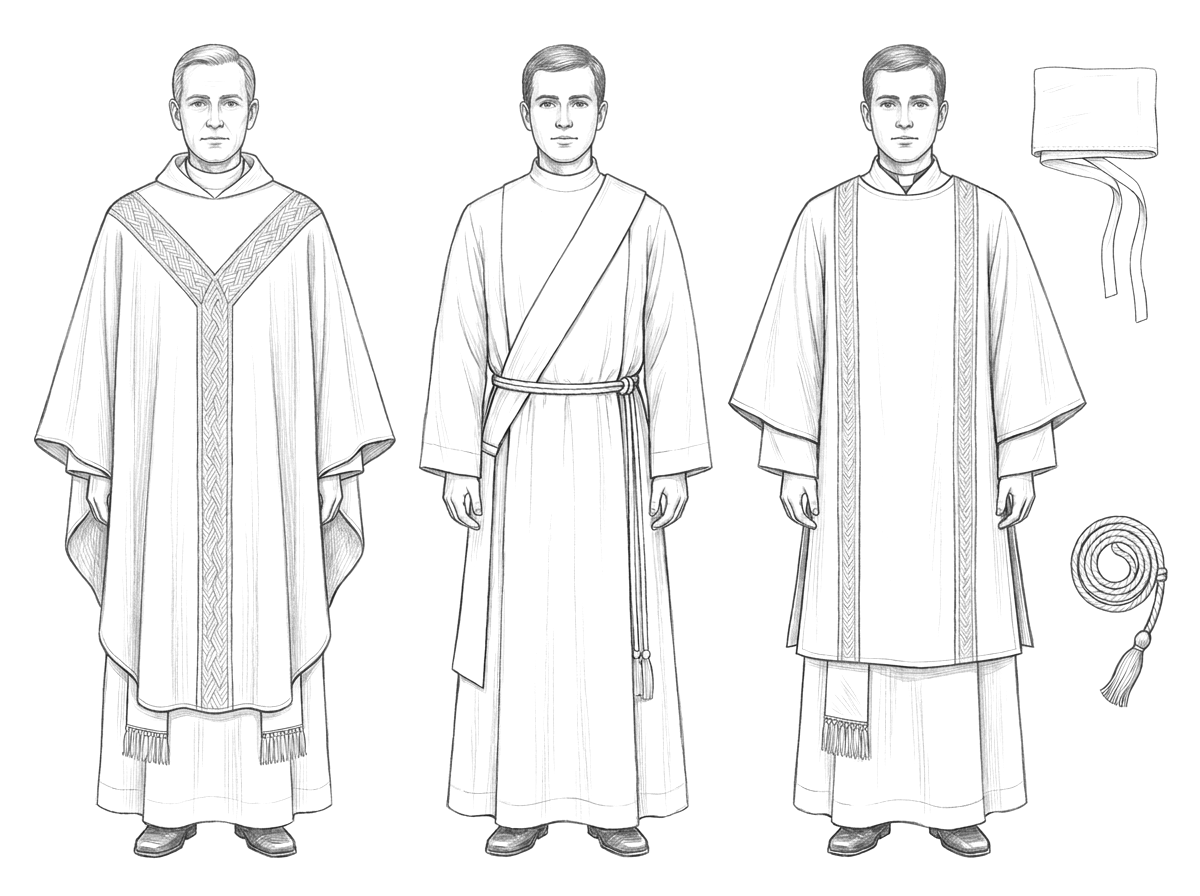
\includegraphics[width=0.92\linewidth,height=3.55in,keepaspectratio]{liturgy/roman-rite/postconciliar/2008-latin-2011-us-english/reference/roman-sanctuary-dictionary/shared/artwork/graphite/pc-art-08-priest-deacon-vesture.png}
\end{center}
\PCDPositionKey{Left: Priest in Alb, Amice, straight vertical Stole, and Y-orphrey Chasuble; center: Deacon in Alb, Cincture, and diagonal Stole from left shoulder to right hip without dalmatic; right: Deacon in Alb and sleeved Dalmatic worn over the diagonal Stole (fringed tip peeking at deacon's right side); far right insets: folded Amice with ties (top) and coiled tasseled Cincture (bottom).}
\else
\textbf{Visual Plate Summary (Plate VIII --- Ordained Vesture at Mass, Standing figures to common scale; insets not to scale):} Worn monochrome graphite vestment study comparing priest and deacon at common scale: left, a priest vested in ankle-length white alb, amice at collar, straight vertical stole ends visible below a flowing Gothic chasuble with Y-shaped orphrey; center, a deacon in white alb and tied cord cincture wearing his stole diagonally from left shoulder across the chest to his right hip; right, a deacon vested in a wide-sleeved dalmatic with vertical clavi stripes worn over the diagonal stole, whose fringed end peeks below the deacon's right hem; far right margin insets show a folded rectangular amice with cloth ties above and a coiled tasseled cincture below.

\textbf{Reading order and object placement:} Left: Priest in Alb, Amice, straight vertical Stole, and Y-orphrey Chasuble; center: Deacon in Alb, Cincture, and diagonal Stole from left shoulder to right hip without dalmatic; right: Deacon in Alb and sleeved Dalmatic worn over the diagonal Stole (fringed tip peeking at deacon's right side); far right insets: folded Amice with ties (top) and coiled tasseled Cincture (bottom).
\fi

\label{pc-obj-alb}
\PCDEntryHead{Alb}{Alba}{required}{N31}
\PCDField{Also called}{White Tunic; \textit{Tunica alba}}
Stock clean, freshly pressed white albs across sizes for clergy, instituted acolytes and lectors, and servers, inspecting hems, collars, and cuffs regularly for wax drips or fraying. Keep clergy albs organized separately from server albs and verify that wide-necked albs are paired with clean amices and cinctures in the sacristy (GIRM 336).

\PCDField{Plate position and norm}{Worn beneath chasuble, diagonal stole, and dalmatic across all three figures (Plate VIII), and under cope and humeral veil (Plate IX) (Universal Roman law)}
\PCDField{Placement and use}{Under universal Roman law, bishops, priests, deacons, instituted acolytes, and instituted lectors wear the alb as their shared liturgical garment (GIRM 336; RS 121--122). It is tied at the waist with a cincture unless tailored to fit neatly without one, and preceded by an amice whenever its neckline leaves ordinary clothing visible at the collar (GIRM 336; Caeremoniale Episcoporum 65). A surplice---even worn over a cassock---may never be substituted for the alb when a chasuble, a dalmatic, or a stole alone is worn (GIRM 336). In the United States, altar servers, readers, and extraordinary ministers of Holy Communion may wear the alb or other dignified clothing approved by diocesan norm (US GIRM 339), but lay ministers never add a stole, dalmatic, or chasuble over it (RS 126).}
\PCDField{United States norm}{While GIRM 336 establishes the alb universally for all ordained and instituted ministers, the USCCB adaptation at GIRM 339 permits acolytes, altar servers, readers, and other lay ministers in the Dioceses of the United States to wear either the alb or other dignified attire suited to liturgical service.}
\PCDField{Prepared and handled by}{Prepares: Sacristan, Altar server. Ministers in use: Bishop, Priest, Deacon, Instituted acolyte, Instituted lector, Extraordinary minister of Holy Communion, Altar server.}
\PCDSafety{Choose an alb whose hem clears your shoes cleanly at ankle height; an overly long hem catches on sanctuary steps and creates a serious tripping hazard, especially when carrying lighted candles, cruets, or a hot thurible.}
\PCDField{Distinguish from}{Cassock and Surplice}
\PCDEntryRule

\label{pc-obj-cincture}
\PCDEntryHead{Cincture}{Cingulum}{required}{N32}
\PCDField{Also called}{Girdle; Waist Cord; \textit{Zona}}
Keep braided cinctures neatly hung or coiled beside the albs so cords do not tangle or fray at the tassels. Provide white cinctures as the standard pairing for clergy and servers, and verify that unfitted albs always have a matching cincture available in the vesting sacristy (GIRM 336).

\PCDField{Plate position and norm}{Tied at waist of center deacon and coiled in lower right inset (Plate VIII) (Universal Roman law)}
\PCDField{Placement and use}{Universal Roman law directs that the alb be secured at the waist with a cincture unless the alb is specifically tailored to fit cleanly without one (GIRM 336; RS 122; Caeremoniale Episcoporum 65). Any bishop, priest, deacon, instituted acolyte, instituted lector, or altar server wearing an unfitted alb ties the cincture smoothly around the waist so that the garment hangs evenly at ankle height. For a deacon serving without a dalmatic, the cincture may also steady the diagonal stole at the waist, whereas the postconciliar priest's straight stole hangs freely over or beside the cincture rather than crossing beneath it (GIRM 340).}
\PCDField{Prepared and handled by}{Prepares: Sacristan, Altar server. Ministers in use: Bishop, Priest, Deacon, Instituted acolyte, Instituted lector, Altar server.}
\PCDSafety{Tie the cincture securely so loose cord ends cannot drag on sanctuary steps, snag on pew corners or candle stands, or brush against open candle flames and hot thuribles.}
\PCDField{Distinguish from}{Stole}
\PCDEntryRule

\label{pc-obj-amice}
\PCDEntryHead{Amice}{Amictus}{required}{N33}
\PCDField{Also called}{Shoulder Cloth}
Keep clean, ironed amices stacked flat in the vesting case beside any wide-necked albs, folding the cloth smoothly with its tie strings coiled neatly inside. Launder amices regularly with ordinary sacristy linens---unlike corporals and purificators, they do not come into contact with the Sacred Species and do not require sacrarium first-rinsing.

\PCDField{Plate position and norm}{At collar of priest on left and folded with tie strings in upper right inset (Plate VIII) (Universal Roman law)}
\PCDField{Placement and use}{Universal Roman law directs that before putting on the alb, a minister is to wear an amice whenever the alb does not completely cover ordinary clothing at the neck (GIRM 336; RS 121--122; Caeremoniale Episcoporum 65). Draped across the shoulders, its tie strings pass under the arms, cross behind the back, and tie in front at the waist before the alb is slipped over it; the folded edge is then turned neatly over the neckline of the alb or chasuble so street or clerical collars remain concealed and outer vestments stay protected from perspiration.}
\PCDField{Prepared and handled by}{Prepares: Sacristan, Altar server. Ministers in use: Bishop, Priest, Deacon, Instituted acolyte, Instituted lector, Altar server.}
\PCDField{Distinguish from}{Corporal, Lavabo Towel}
\PCDEntryRule

\label{pc-obj-stole}
\PCDEntryHead{Stole}{Stola}{required}{N34}
\PCDField{Also called}{Priestly Stole; Diaconal Stole}
Lay out the matching seasonal priestly stole with every chasuble and the matching diaconal stole (tailored to fasten cleanly at the right hip) with every dalmatic, checking GIRM 346 and the United States color options for funerals and solemnities (US GIRM 346e, 346h). Hang stoles flat or draped cleanly without creasing embroidered orphreys, and keep a violet and white sacramental stole ready for Confessions and pastoral visits.

\PCDField{Plate position and norm}{Hanging straight below priest's chasuble at left; worn diagonally from left shoulder to right hip on center deacon and beneath right deacon's dalmatic with tip peeking at his right hem (Plate VIII) (Universal Roman law)}
\PCDField{Placement and use}{At Mass, the priest wears the stole around his neck hanging straight down in front of his chest---not crossed over the breast---over the alb and beneath the chasuble, matching the bishop's manner (GIRM 337, 340). The deacon wears the stole diagonally from his left shoulder across his chest and back to be fastened at his right side, always beneath the dalmatic when the dalmatic is worn (GIRM 338, 340). A priest or deacon may never celebrate Mass wearing only a stole over ordinary street clothes or a monastic habit without the alb and appointed outer vestment, nor may a surplice replace the alb when only a stole is worn (GIRM 336; RS 123--126). Laypersons---including instituted acolytes, instituted lectors, extraordinary ministers of Holy Communion, and altar servers---are strictly prohibited from wearing a stole (RS 126). The stole follows the seasonal color of the day (GIRM 346): white, red, green, violet, rose (Gaudete and Laetare Sundays), black where customary, or festive gold or silver in the United States.}
\PCDField{United States norm}{While the stole's wearing and reservation to ordained ministers follow universal Roman law (GIRM 340; RS 123--126), USCCB adaptations at GIRM 346e and 346h permit white, violet, or black stoles for funerals and Masses for the Dead, and gold or silver stoles on more solemn occasions.}
\PCDField{Prepared and handled by}{Prepares: Sacristan. Ministers in use: Bishop, Priest, Deacon.}
\PCDField{Distinguish from}{Cincture, Humeral Veil}
\PCDEntryRule

\label{pc-obj-chasuble}
\PCDEntryHead{Chasuble}{Casula}{required}{N35}
\PCDField{Also called}{Mass Vestment; \textit{Planeta}}
Lay out a clean, blessed chasuble of the appointed liturgical color (GIRM 335, 346; US 346e, 346h) paired with its matching priestly stole over wide contoured hangers so the shoulders never crease. For concelebrated Masses, prepare matching chasubles for concelebrants wherever available, reserving omission solely for genuine necessity (GIRM 209; RS 124).

\PCDField{Plate position and norm}{Left figure, Y-orphrey outer vestment of priest celebrant (Plate VIII) (Universal Roman law)}
\PCDField{Placement and use}{Unless the rubrics provide otherwise, the chasuble is always worn by the priest celebrant---and by the principal celebrant at a concelebrated Mass---over the alb and stole at Mass and during actions directly connected with Mass, such as the Sunday sprinkling rite, Ash Wednesday imposition of ashes, and the final commendation at a funeral Mass (GIRM 337; RS 123; Tres abhinc annos 26). Concelebrating priests other than the principal celebrant wear the chasuble as well, omitting it only for a just reason such as a large gathering of priests or a scarcity of vestments, in which case they wear the stole over the alb (GIRM 209; RS 124). Deacons, instituted ministers, extraordinary ministers of Holy Communion, and altar servers never wear a chasuble (RS 126). Its nobility derives from quality fabric and graceful form rather than lavish ornament (GIRM 344), following the seasonal color cycle of GIRM 346.}
\PCDField{United States norm}{While universal Roman law requires the chasuble for the priest celebrant at Mass (GIRM 337; RS 123--124), USCCB adaptations at GIRM 346e and 346h permit white, violet, or black chasubles at funeral Masses and Masses for the Dead, and gold or silver chasubles on more solemn occasions.}
\PCDField{Prepared and handled by}{Prepares: Sacristan. Ministers in use: Bishop, Priest.}
\PCDField{Distinguish from}{Dalmatic, Cope}
\PCDEntryRule

\label{pc-obj-dalmatic}
\PCDEntryHead{Dalmatic}{Dalmatica}{provided}{N36}
\PCDField{Also called}{Deacon's Dalmatic; \textit{Dalmatica diaconalis}}
Lay out a clean dalmatic matching the seasonal color of the celebrant's chasuble whenever a deacon ministers at Mass (GIRM 338, 346; RS 125), paired with a diaconal stole, alb, and cincture as needed. Verify that wide sleeves and side fastenings are neat and uncreased, and keep a lightweight pontifical dalmatic ready when the diocesan bishop celebrates major solemnities (CE 1984 no. 56).

\PCDField{Plate position and norm}{Right figure, wide-sleeved rectangular outer vestment worn over the diagonal stole (Plate VIII) (Universal Roman law)}
\PCDField{Placement and use}{At Mass, the deacon vests in the alb (with amice and cincture as needed), puts on the stole diagonally from his left shoulder to his right hip, and wears the dalmatic over the stole---never the stole on top of the dalmatic (GIRM 336, 338, 340). Although GIRM 338 permits the dalmatic to be omitted out of necessity or on account of a lesser degree of solemnity, Redemptionis Sacramentum 125 commends keeping the dalmatic in regular use rather than routinely omitting it. On major solemnities and pontifical Masses, a bishop may also wear a lightweight pontifical dalmatic beneath his chasuble (Caeremoniale Episcoporum 1984 no. 56). Lay ministers---including instituted acolytes and altar servers---never wear a dalmatic (RS 126).}
\PCDField{United States norm}{Universal Roman law appoints the dalmatic as the proper vestment of the deacon (GIRM 338), permitting omission out of necessity or on lesser occasions while Redemptionis Sacramentum 125 praises refraining from omitting it; United States GIRM 346e and 346h govern funeral and solemnity color options.}
\PCDField{Prepared and handled by}{Prepares: Sacristan. Ministers in use: Deacon, Bishop.}
\PCDField{Distinguish from}{Chasuble, Subdeacon's Tunicle and Maniple}
\PCDEntryRule

\clearpage
\PCDPlateHeader{Plate IX --- Choir Dress and Solemn Ceremonial Vesture}{Standing figures to common scale}
\ifdefined\TriptychPrintEdition
\begin{center}
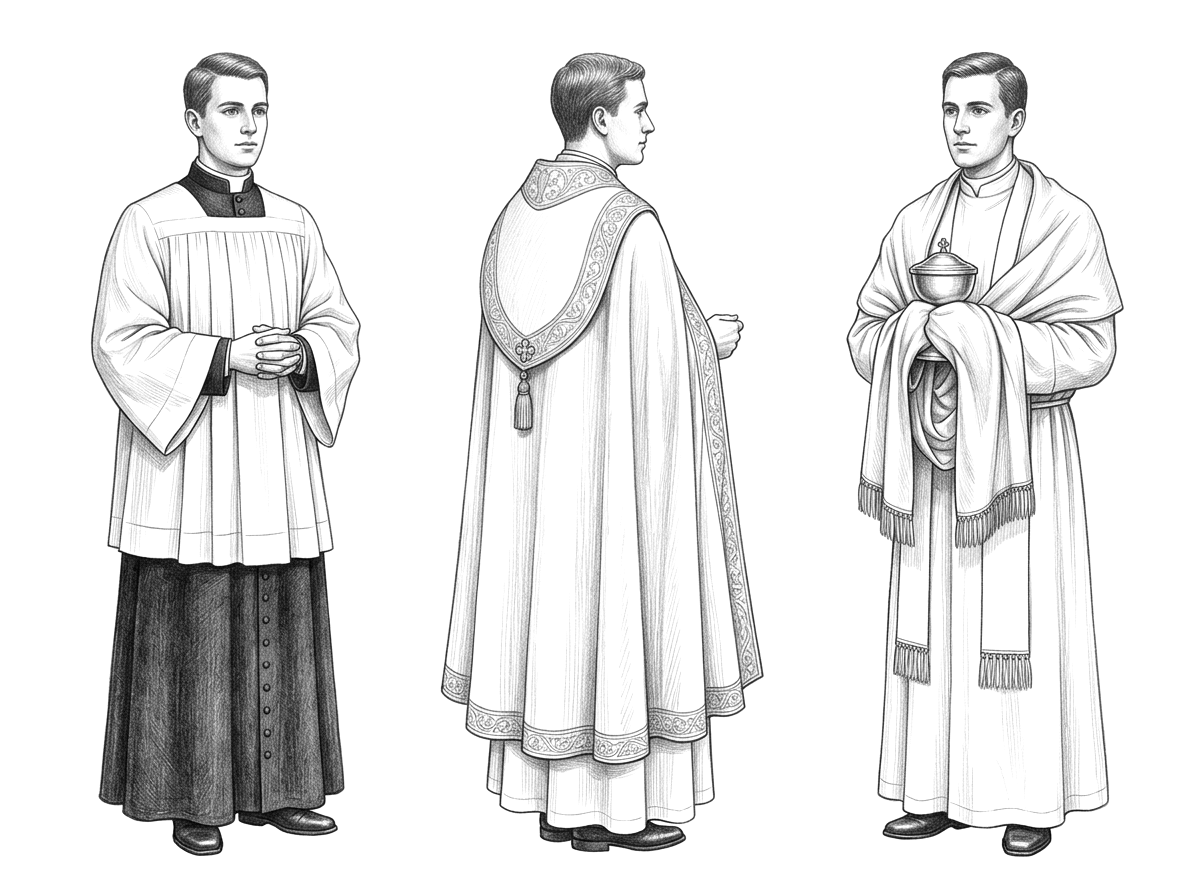
\includegraphics[width=0.92\linewidth,height=3.55in,keepaspectratio]{liturgy/roman-rite/postconciliar/2008-latin-2011-us-english/reference/roman-sanctuary-dictionary/shared/artwork/graphite/pc-art-09-black-cassock-surplice-cope.png}
\end{center}
\PCDPositionKey{Left: choir dress (deep black buttoned clerical Cassock beneath crisp white pleated Surplice); center: three-quarter rear view of semicircular Cope with ornamental hood shield and tassel over an Alb; right: Priest in Alb and straight Stole wearing a fringed Humeral Veil whose cloth completely envelops both hands supporting a closed lidded ciborium.}
\else
\textbf{Visual Plate Summary (Plate IX --- Choir Dress and Solemn Ceremonial Vesture, Standing figures to common scale):} Three-figure monochrome graphite garment study demonstrating high-contrast shading: left, a standing figure in clerical choir dress wearing a deep charcoal-black ankle-length buttoned cassock under a bright white pleated wide-sleeved surplice; center, three-quarter rear view of a flowing semicircular cope with embroidered hood shield and tassel worn over a white alb; right, three-quarter front view of a priest in alb and straight vertical stole draped in an oblong fringed humeral veil whose ends wrap completely over both hands as he holds a closed lidded ciborium.

\textbf{Reading order and object placement:} Left: choir dress (deep black buttoned clerical Cassock beneath crisp white pleated Surplice); center: three-quarter rear view of semicircular Cope with ornamental hood shield and tassel over an Alb; right: Priest in Alb and straight Stole wearing a fringed Humeral Veil whose cloth completely envelops both hands supporting a closed lidded ciborium.
\fi

\label{pc-obj-cassock-surplice}
\PCDEntryHead{Cassock and Surplice}{Vestis talaris et superpelliceum}{permitted}{N37}
\PCDField{Also called}{Choir Dress; Server's Cassock and Surplice; \textit{Talaris}; \textit{Superpelliceum}; \textit{Cotta}}
Maintain a graded size rack of clean black cassocks and pressed white surplices for servers and choir clergy (RS 128; US GIRM 339), keeping missing buttons repaired and hems intact to prevent tripping hazards. Remember that priests celebrating or concelebrating Mass or vesting in a stole under GIRM 336 require an alb---never substitute a surplice over a cassock for the alb at Mass.

\PCDField{Plate position and norm}{Left figure, deep charcoal-black ankle-length buttoned cassock under bright pleated white surplice (Plate IX) (Universal Roman law)}
\PCDField{Placement and use}{In postconciliar discipline, two sharp rules govern cassock and surplice. First, the alb may never be exchanged for a surplice, not even over a cassock, when a chasuble or dalmatic is worn or when rubrics prescribe only a stole without an outer vestment (GIRM 336; CE 1984 no. 65). Second, whenever a surplice is worn, it must always be worn over a cassock---never directly over ordinary street clothing (CE 1984 no. 65). Non-concelebrating priests attending Mass in choir wear choir dress or a surplice over a cassock (Redemptionis Sacramentum 128). For altar servers in the United States, cassock and surplice remain a widely esteemed, dignified traditional alternative to the white alb (US GIRM 339).}
\PCDField{United States norm}{Under the United States adaptation to GIRM 339, altar servers, acolytes, readers, and other lay ministers may wear either the alb or other appropriate and dignified clothing such as cassock and surplice. Universal law strictly forbids substituting a surplice over a cassock for the alb whenever a chasuble, dalmatic, or stole alone is worn (GIRM 336), and requires that a surplice always be worn over a cassock (Caeremoniale Episcoporum 1984 no. 65).}
\PCDField{Prepared and handled by}{Prepares: Sacristan, Altar server. Ministers in use: Bishop, Priest, Deacon, Instituted acolyte, Altar server.}
\PCDSafety{Ensure the cassock hem clears the floor cleanly above the shoes so it does not catch on sanctuary steps while carrying candles, the processional cross, or a smoking thurible; never wear a surplice without a cassock underneath (CE 1984 no. 65).}
\PCDField{Distinguish from}{Alb}
\PCDEntryRule

\label{pc-obj-cope}
\PCDEntryHead{Cope}{Pluviale}{provided}{N38}
\PCDField{Also called}{Processional Mantle; \textit{Cappa}}
Prepare the white cope paired with a matching white stole and humeral veil for Eucharistic Benediction and Corpus Christi processions (HCWEOM nn. 91--92), and seasonal copes for Palm Sunday processions or Solemn Liturgy of the Hours (GIRM 341). Check that the front clasp (morse) closes securely before vesting, and store copes flat or on wide curved hangers to prevent shoulder creases.

\PCDField{Plate position and norm}{Center figure, three-quarter rear view showing full semicircular cloak, embroidered hood shield, and tassel over an alb (Plate IX) (Universal Roman law)}
\PCDField{Placement and use}{GIRM 341 specifies that the cope is worn by the priest in processions and during other sacred actions in accordance with the rubrics proper to individual rites---such as Solemn Benediction with the monstrance (where a white cope and humeral veil are prescribed: Holy Communion and Worship of the Eucharist Outside Mass nn. 91--92), Eucharistic processions, Solemn Liturgy of the Hours, solemn blessings, and funeral rites outside Mass. A priest never celebrates the Mass itself in a cope: if worn for an entrance procession such as Palm Sunday, he exchanges it for the chasuble before beginning the Mass prayers (GIRM 337, 341). A deacon wears the cope only when presiding at specific non-Mass rites such as Solemn Benediction or Solemn Vespers.}
\PCDField{United States norm}{GIRM 341 governs the cope universally according to the rubrics of individual rites; United States GIRM 346e and 346h apply to funeral and festive gold/silver color choices.}
\PCDField{Prepared and handled by}{Prepares: Sacristan, Altar server. Ministers in use: Bishop, Priest, Deacon.}
\PCDSafety{When holding the edges of a priest's or bishop's cope during incensation or procession, keep the heavy front fabric well clear of lighted candles and hot thurible chains, and unfasten the chest clasp gently without tugging delicate embroidery.}
\PCDField{Distinguish from}{Chasuble, Humeral Veil}
\PCDEntryRule

\label{pc-obj-humeral-veil}
\PCDEntryHead{Humeral Veil}{Velum humerale}{provided}{N39}
\PCDField{Also called}{Benediction Veil; \textit{Velum}}
Lay out a clean, pressed white humeral veil beside the credence table or sanctuary steps before Eucharistic Benediction, Corpus Christi processions, and the Holy Thursday Evening Mass of the Lord's Supper (HCWEOM nn. 91--92). Check that its front ribbon ties or metal clasp work smoothly and that interior hand-pockets (if tailored) are clean and unripped. Keep episcopal vimpas labeled separately from the Eucharistic humeral veil.

\PCDField{Plate position and norm}{Right figure, oblong fringed white cloth draped over shoulders with ends wrapping completely over both hands around a lidded ciborium (Plate IX) (Universal Roman law)}
\PCDField{Placement and use}{The Eucharistic humeral veil is required whenever a bishop, priest, or deacon imparts Benediction with the monstrance (over a white cope) or with a ciborium, carries the Blessed Sacrament in a solemn procession (such as Corpus Christi), or transfers the Blessed Sacrament to the altar of reposition at the close of the Holy Thursday Evening Mass of the Lord's Supper (Holy Communion and Worship of the Eucharist Outside Mass nn. 91--92; Roman Missal, Holy Thursday). Extraordinary ministers of Holy Communion and altar servers never impart Eucharistic Benediction and never wear the Eucharistic humeral veil. Distinguish the Eucharistic humeral veil from the narrower vimpa worn by miter- and crosier-bearers during pontifical liturgies (Caeremoniale Episcoporum 1984).}
\PCDField{Prepared and handled by}{Prepares: Sacristan, Altar server. Ministers in use: Bishop, Priest, Deacon.}
\PCDSafety{Fasten the front clasp cleanly and evenly without pulling the priest's stole or collar, and ensure the long fringed ends do not brush against lighted candles on the altar steps while the celebrant ascends to lift the monstrance or ciborium.}
\PCDField{Distinguish from}{Cope, Stole}
\PCDEntryRule
